% !TEX TS-program = pdflatex
% !TEX encoding = UTF-8 Unicode

\documentclass[11pt]{article} % use larger type; default would be 10pt

\usepackage{pgf}
\usepackage{tikz}
\usetikzlibrary{arrows,automata,shapes}
\usetikzlibrary{decorations.pathmorphing} % LATEX and plain TEX when using Tik Z

\usepackage[utf8]{inputenc} % set input encoding (not needed with XeLaTeX)

%%% PAGE DIMENSIONS
\usepackage{geometry} % to change the page dimensions
\geometry{a4paper} % or letterpaper (US) or a5paper or....
\geometry{margin=2cm} % for example, change the margins to 2 inches all round
% \geometry{landscape} % set up the page for landscape
%   read geometry.pdf for detailed page layout information

\usepackage{graphicx} % support the \includegraphics command and options
\usepackage{subcaption} % for subfigures

\usepackage{scrextend} % https://tex.stackexchange.com/questions/588/how-can-i-change-the-margins-for-only-part-of-the-text
\usepackage{color}
\definecolor{rowcolor}{rgb}{0.94, 0.97, 1.0}  % 1=weiß, 0=schwarz

% \usepackage[parfill]{parskip} % Activate to begin paragraphs with an empty line rather than an indent

%%% PACKAGES
\usepackage{booktabs} % for much better looking tables
\usepackage{array} % for better arrays (eg matrices) in maths
\usepackage{paralist} % very flexible & customisable lists (eg. enumerate/itemize, etc.)
\usepackage{verbatim} % adds environment for commenting out blocks of text & for better verbatim
%\usepackage{subfig} % make it possible to include more than one captioned figure/table in a single float
% These packages are all incorporated in the memoir class to one degree or another...
\usepackage{listings} % Absatz als Code formatieren
\usepackage{floatflt} % für floatingfigure

%%% HEADERS & FOOTERS
\usepackage{fancyhdr} % This should be set AFTER setting up the page geometry
\pagestyle{fancy} % options: empty , plain , fancy
\renewcommand{\headrulewidth}{0pt} % customise the layout...
\lhead{Driver for Vector Signal Generator}\chead{User documentation}\rhead{\today}
\lfoot{M.Wagener / S.Fleitmann}\cfoot{\thepage}\rfoot{FZJ/ZEA-2}

%%% SECTION TITLE APPEARANCE
\usepackage{sectsty}
\allsectionsfont{\sffamily\mdseries\upshape} % (See the fntguide.pdf for font help)
% (This matches ConTeXt defaults)

%%% ToC (table of contents) APPEARANCE
\usepackage[nottoc,notlof,notlot]{tocbibind} % Put the bibliography in the ToC
\usepackage[titles,subfigure]{tocloft} % Alter the style of the Table of Contents
\renewcommand{\cftsecfont}{\rmfamily\mdseries\upshape}
\renewcommand{\cftsecpagefont}{\rmfamily\mdseries\upshape} % No bold!

\usepackage{longtable} % Tabellen über mehrere Seiten
\usepackage{multirow} % multirow/multicolumn
\usepackage{colortbl} % farbige Tabellenzellen
\setlength{\LTpre}{0pt}  % Remove whitespace befor and after longtables
\setlength{\LTpost}{0pt}

\setlength{\tabcolsep}{1mm} % Setzt den Längenwert von {Abstand zwischen den Spalten einer Tabelle} auf den Wert 1mm
\setcounter{tocdepth}{2}  % Tiefe des Inhaltsverzeichnisses

\setlength{\parindent}{0em} % Damit die neuen Absätze nicht eingerückt werden

%%% END Article customizations

%%% The "real" document content comes below...

\title{QCoDeS driver for the Rohde\&Schwarz Vector Signal Generator \newline {\it User documentation}}
\author{Michael Wagener / Sarah Fleitmann, FZJ/ZEA-2}

\begin{document}
\maketitle

\tableofcontents % toc anzeigen

\ \\

\begin{longtable}{|p{2.7cm}|p{2.6cm}|p{10.3cm}|}
\caption{Document revision history} \\
\hline\rowcolor{rowcolor}{\bf Date} & {\bf Author} & {\bf Short description} \\
\endfirsthead
\hline
07. Jun 2019 & M.Wagener & First edit phase. \\ \hline
14. Jun 2019 & M.Wagener & Continue editing the classes and parameters. \\ \hline
19. Jun 2019 & M.Wagener & Fixup formatting. \\ \hline
24. Jun 2019 & M.Wagener & Last corrections. \\ \hline
01. Aug 2019 & M.Wagener & Short descriptions of test scripts. \\ \hline
29. Jan. 2020 & M.Wagener & Add genTriggerPulse() function. \\ \hline
\end{longtable}


\clearpage

%%%
\section{Informations}

\begin{floatingfigure}[r]{0.42\textwidth}
\mbox{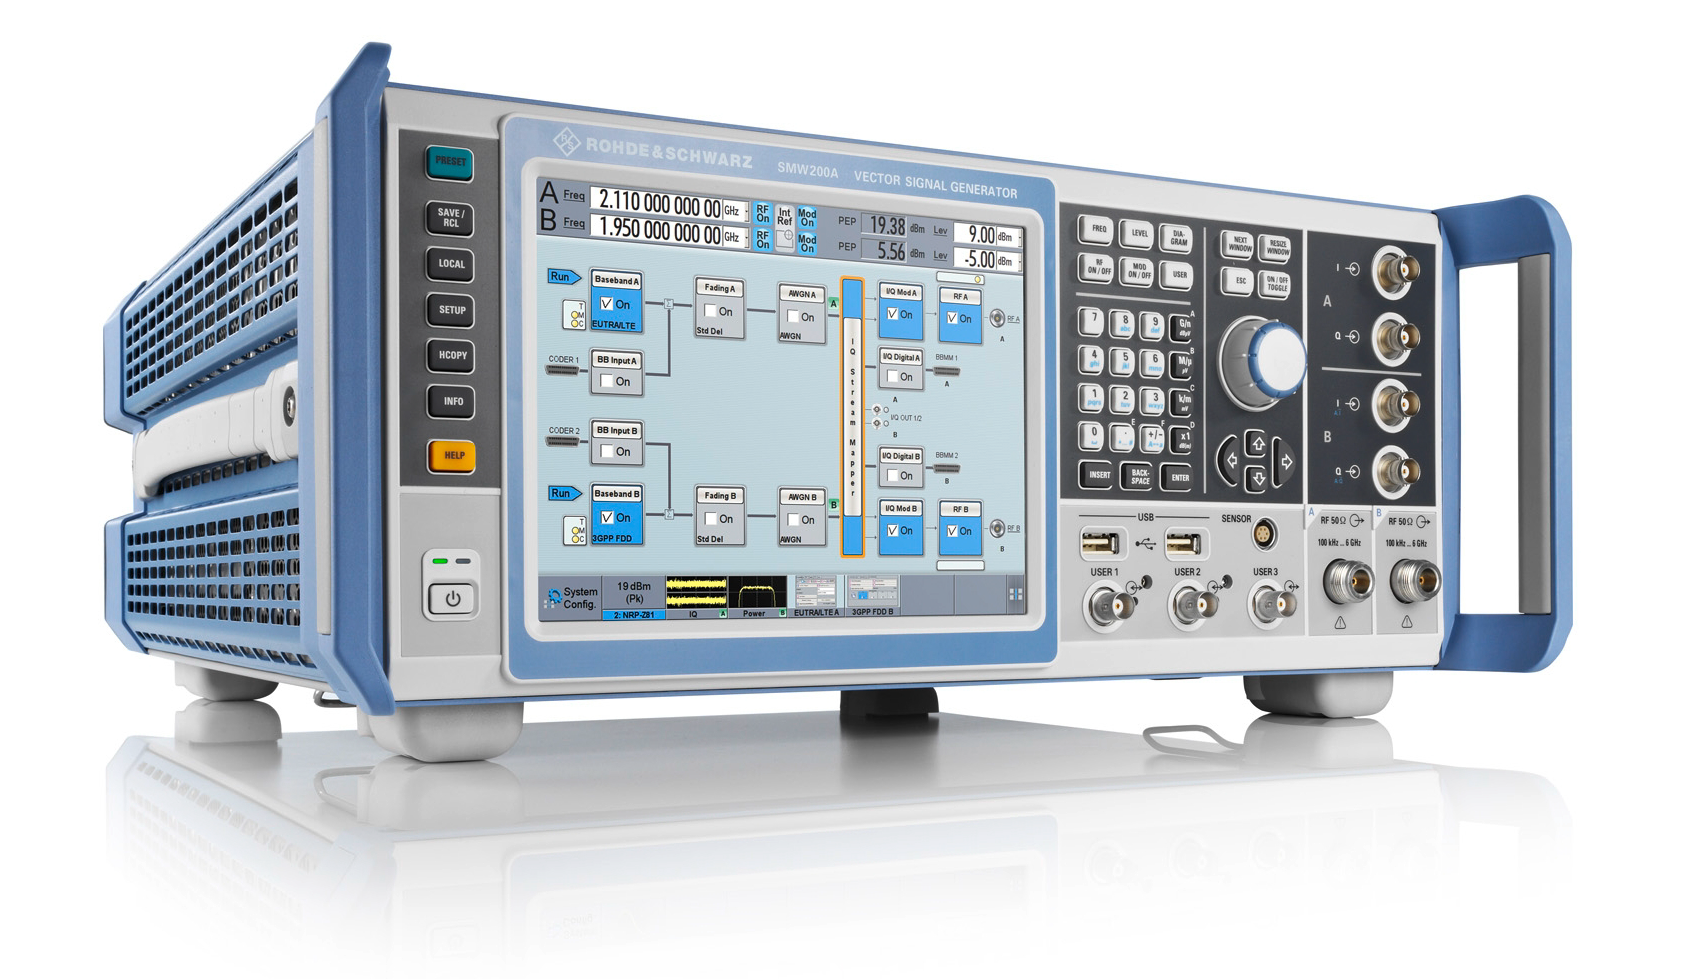
\includegraphics[width=0.4\textwidth]{DeviceFromHandbook.png}}
\caption{Picture from device manual}
\end{floatingfigure}
This manual describes the QCoDeS driver for the Rohde\&Schwarz Vector Signal Generator SMW200A.
It can generate a number of signaltypes with different modulations.

\ \\

This manual describes the implemented classes and their parameters to be used	 in the QCoDeS environment. Some parameters can only be used with special installed options. This will be noted here. If the parameters require an option which was not installed at our test device, then we can only write the informations from the device manual. These commands are not tested.

\ \\

\subsection{Git and directories}

The software will be saved in the RWTH git system.

\ \\

% Dieses Absatz kann später eventuell wieder raus
During development the software will be saved in the local ZEA-2 git system:
\begin{itemize}
\item Source and Test-Scripts \\
	{\it zea2git.zel.kfa-juelich.de:Quantencomputing/devices/SMW200A.git}
\item User-Documentation, Development logbook and Requirement specifications \\
	{\it zea2git.zel.kfa-juelich.de:Quantencomputing/Dokumentation.git} \\
	{\small (This directory was used for all driver documentation.)}
\end{itemize}


\clearpage


%%%
\section{General usage}

This short example shows the first steps with this driver. Important is the correct IP address for the device. This example will print the identification string and the list of installed options. These options can change the amount of parameters. The last command {\it dev.close()} is only important if you want to connect to the device again with the {\it smw200a(...)} constructor.

\begin{lstlisting}[frame=single, language=Python]
> from qcodes.instrument_drivers.rohde_schwarz.SMW200A
			import RohdeSchwarz_SMW200A as smw200a
> dev = smw200a( name='SMW200A',
                 address='TCPIP::134.61.7.134::hislip0::INSTR' )
> print( "ID:", dev.get_id() )
ID: Rohde&Schwarz,SMW200A,1412.0000K02/105578,04.30.005.29 SP2
> print( "Options:", dev.get_options() )
Options: ['SMW-B13T', 'SMW-B22', 'SMW-B120', 'SMW-K22']
> dev.close()
\end{lstlisting}


\section{Class documentation}

Here is a list of all defined classes and their defined parameters in the same order as they appear in the source code.


\subsection{IQChannel}

The I/Q channels are the analog output channels of the device.
\begin{itemize}
\item {\bf state()} Actives/deactives the I/Q output. Values are 'ON' and 'OFF'.
\item {\bf type()} Sets the type of the analog signal. Values are 'SING' (single) and 'DIFF' (differential, {\it only available with option SMW-K16})
\item {\bf mode()} Determines the mode for setting the output parameters. Values are 'FIX' (locks the I/Q output settings) and 'VAR' (unlocks the settings, {\it only available with option SMW-K16})
\item {\bf level()} Sets the off-load voltage Vp of the analog I/Q signal output. Values are in range 0.04V to 4V for option SMW-B10 and in range 0.04V to 2V for option SMW-B9. The value range is adjusted so that the maximum overall output voltage does not exceed 4V. {\it This is only settable when mode() has the value 'VAR' and so the option `SMW-K16' is installed.}
\item {\bf coupling()} Couples the bias setting of the I and Q signal components. Values are 'ON' and 'OFF'.
\item {\bf i\_bias()}$^{(*)}$ Specifies the amplifier bias of the I component.
\item {\bf q\_bias()}$^{(*)}$ Specifies the amplifier bias of the Q component.
\item {\bf i\_offset()}$^{(*)}$ Sets an offset between the inverting and non-inverting input of the differential analog I/Q output signal for the I component.
\item {\bf q\_offset()}$^{(*)}$ Sets an offset between the inverting and non-inverting input of the differential analog I/Q output signal for the Q component.
\item[] $^{(*)}$ The value ranges of these parameters dependent on each other and the value of level(). So they are adjusted to the maximum overall output voltage of 4V. {\it They are only settable when mode() has the value 'VAR' and so the option `SMW-K16' is installed.}
\end{itemize}


\subsection{IQModulation}

Combines all the parameters concerning the I/Q modulation.
\begin{itemize}
\item {\bf state()} Activates/deactivates the I/Q modulation. Values are 'ON', and 'OFF'
\item {\bf source()} Selects/reads the input signal source for the I/Q modulator. Values are:
	\begin{itemize}[]
	\item 'BAS': internal baseband signal
	\item 'ANAL': external Analog Wideband I/Q Input signal 
	\item 'DIFF': differential analog signal ({\it only with option SMW-K739})
	\end{itemize}
\item {\bf gain()} Optimizes the modulation of the I/Q modulator for a subset of measurement requirements. Values are:
	\begin{itemize}[]
	\item 'DB0', 'DB2', 'DB4', 'DB6', 'DB8': \\
		Activates the specified gain of 0 dB, +2 dB, +4 dB, +6 dB, +8 dB
	\item 'DBM2', 'DBM4': \\
		Activates the specified gain of -2 dB, -4 dB
	\item 'DBM3', 'DB3': \\
		Provided only for backward compatibility with other Rohde \& Schwarz signal generators. The R\&S SMW accepts these values and maps them automatically as follows: DBM3 = DBM2, DB3 = DB2
	\item 'AUTO': \\
		The gain value is retrieved form the connected R\&S SZU\footnote{External Frequency Converter / Externally connected R\&S SZU IQ Upconverter}. The I/Q modulator is configured automatically.
	\end{itemize}
\item {\bf crest\_factor()} If source set to `ANAL' (Analog Wideband I/Q Input), sets the crest factor of the externally supplied analog signal. The crest factor gives the difference in level between the peak envelope power (PEP) and the average power value (RMS) in dB. The R\&S SMW uses this value for the calculation of the RF output power. The allowed range is from 0 dB to 35 dB.
\item {\bf swap()} Activates/Deactives the swapping of the I and Q channel. Values are 'ON' and 'OFF'.
\item {\bf wideband()} Actives/Deactivates the wideband mode. Values are 'ON' and 'OFF'.
\end{itemize}


\subsection{FrequencyModulation}

Combines all the parameters concerning the frequency modulation.
\begin{itemize}
\item {\bf state()} Actives/deactivates the frequency modulation. Values are 'ON' and 'OFF'.
\item {\bf deviation()} Sets the modulation deviation of the frequency modulation in Hz.
\item {\bf source()} Selects the modulation source. Values are:
	\begin{itemize}[]
	\item 'INT': equals 'LF1' ({\it for channel 2 only available with option SMW-K24})
	\item 'EXT': equals 'EXT1' ({\it for channel 2 only available with option SMW-K24})
	\item 'LF1': first internally generated signal
	\item 'LF2': second internally gererated signal ({\it only available with option SMW-K24})
	\item 'NOIS': internally generated noise signal ({\it only available with option SMW-K24})
	\item 'EXT1': first externally supplied signal
	\item 'EXT2': second externally supplied signal
	\item 'INTB': internal baseband signal ({\it only available with option SMW-B9})
	\end{itemize}
\item {\bf coupling\_mode()} Selects the coupling mode. The coupling mode parameter also determines the mode for fixing the total deviation. Possible Values are:
	\begin{itemize}[]
	\item 'UNC': Does not couple the LF signals. The deviation values of both paths are independent. This is the default after reset.
	\item 'TOT': Couples the deviation of both paths in per Hz. If you change the deviation of any path, the R\&S SMW automatically adjusts the value of the other path. The sum always results in the set Total Deviation.
	\item 'RAT': Couples the deviation ratio of both paths. If you change the deviation of any path, the R\&S SMW adjusts the value of the other path.
	\end{itemize}
	{\it This parameter was not working on the test device but there is no hint to an option to install in the manual. So this parameter will be hidden in the current version.}
\item {\bf total\_deviation()} Sets the total deviation of the LF signal when using combined signal sources in frequency modulation.
	{\it This parameter was not working on the test device but there is no hint to an option to install in the manual. So this parameter will be hidden in the current version.}
\item {\bf deviation\_ratio()} Sets the deviation ratio (path2 to path1) in percent.
\item {\bf mode()} Selects the mode for the frequency modulation. Values are 'NOR' (normal mode) and 'LNO' (low noise mode)
\item {\bf sensitivity()} {\it (ReadOnly)} Queries the sensitivity of the externally supplied signal for frequency modulation in Hz/V. The sensitivity depends on the set modulation deviation.
\end{itemize}


\subsection{AmplitudeModulation}

Combines all the parameters concerning the amplitude modulation.
Activation of amplitude modulation deactivates ARB, I/Q modulation, digital modulation and all digital standards.
\begin{itemize}
\item {\bf state()} Actives/deactivates the amplitude modulation. Values are 'ON' and 'OFF'.
\item {\bf source()} Selects the modulation source. Values are:
	\begin{itemize}[]
	\item 'INT': equals 'LF1' ({\it for channel 2 only available with option SMW-K24})
	\item 'EXT': equals 'EXT1' ({\it for channel 2 only available with option SMW-K24})
	\item 'LF1': first internally generated signal
	\item 'LF2': second internally generated signal ({\it only available with option SMW-K24})
	\item 'NOIS': internally generated noise signal ({\it only available with option SMW-K24})
	\item 'EXT1': first externally supplied signal
	\item 'EXT2': second externally supplied signal
	\end{itemize}
\item {\bf depth()} Sets the depth of the amplitude modulation in percent (0 to 100).
\item {\bf total\_depth()} Sets the total depth of the LF signal when using combined signal sources in amplitude modulation.
	{\it This parameter was not working on the test device but there is no hint to an option to install in the manual. So this parameter will be hidden in the current version.}
\item {\bf coupling\_mode()} Selects the coupling mode. The coupling mode parameter also determines the mode for fixing the total depth. Values are:
	\begin{itemize}[]
	\item 'UNC': Does not couple the LF signals. The deviation values of both paths are independent. This is the default after reset.
	\item 'TOT': Couples the deviation of both paths in per Hz. If you change the deviation of any path, the R\&S SMW automatically adjusts the value of the other path. The sum always results in the set Total Deviation.
	\item 'RAT': Couples the deviation ratio of both paths. If you change the deviation of any path, the R\&S SMW adjusts the value of the other path.
	\end{itemize}
	{\it This parameter was not working on the test device but there is no hint to an option to install in the manual. So this parameter will be hidden in the current version.}
\item {\bf deviation\_ratio()} Sets the deviation ratio (path2 to path1) in percent.
\item {\bf sensitivity()} {\it (ReadOnly)} Queries the sensitivity of the externally applied signal. The sensitivity depends on the set modulation depth. The returned value reports the sensitivity in \%/V. It is assigned to the voltage value for full modulation of the input.
\end{itemize}


\subsection{PulseModulation}

Combines all the parameters concerning the pulse modulation.
\begin{itemize}
\item {\bf state()} Activates/deactivates the pulse modulation. Values are 'ON' and 'OFF'.
\item {\bf source()} Selects the modulation source. Values are:
	\begin{itemize}[]
	\item 'INT': internally generated signal is used ({\it only available with option SMW-K23})
	\item 'EXT': externally supplied signal is used
	\end{itemize}
\item {\bf transition\_type()} sets the transition mode for the pulse signal. Values are:
	\begin{itemize}[]
	\item 'SMO': flattens the slew, resulting in longer rise/fall times (SMOothed)
	\item 'FAST': enables fast transition with shortest rise and fall times
	\end{itemize}
\item {\bf video\_polarity()} Sets the polarity of the pulse video (modulating) signal, related to the RF (modulated) signal. Values are:
	\begin{itemize}[]
	\item 'NORM': the video signal follows the RF signal, that means it is high when RF signal is high and vice versa
	\item 'INV': the video signal follows in inverted mode
	\end{itemize}
\item {\bf polarity()} Sets the polarity of the externally applied modulation signal. Values are:
	\begin{itemize}[]
	\item 'NORM': Suppresses the RF signal during the pulse pause
	\item 'INV': Suppresses the RF signal during the pulse
	\end{itemize}
\item {\bf impedance()} Sets the impedance for the external pulse modulation input. Values are 'G50' and 'G1K'.
\item {\bf trigger\_impedance()} Sets the impedance for the external pulse trigger. Values are 'G50' and 'G10K'
\item[] {\it The following parameters are only available with option SMW-K23}
\item {\bf mode()} Selects the mode for the pulse modulation. Values can be 'SING' for a single pulse and 'DOUB' for two pulses within one pulse period.
\item {\bf double\_delay()} Sets the delay from the start of the first pulse to the start of the second pulse
\item {\bf double\_width()} Sets the width of the second pulse
\item {\bf trigger\_mode()} Selects a trigger mode for generating the modulation signal. Values are 'AUTO' (AUTOmatic), 'EXT' (EXTernal), 'EGAT' (External GATed), 'ESIN' (External SINgle)
\item {\bf period()} Sets the period of the generated pulse, that means the repetition frequency of the internally generated modulation signal.
\item {\bf width()} Sets the width of the generated pulse, that means the pulse length. It must be at least 20ns less than the set pulse period.
\item {\bf delay()} Sets the pulse delay.
\end{itemize}


\subsection{PhaseModulation}

Combines all the parameters concerning the phase modulation.
\begin{itemize}
\item {\bf state()} Activates/deactivates phase modulation. Activation of phase modulation deactivates frequency modulation. Possible values are 'ON' and 'OFF'.
\item {\bf deviation()} Sets the modulation deviation of the phase modulation in RAD.
\item {\bf source()} Selects the modulation source. Values are:
	\begin{itemize}[]
	\item 'INT': equals 'LF1' ({\it for channel 2 only available with option SMW-K24})
	\item 'EXT': equals 'EXT1' ({\it for channel 2 only available with option SMW-K24})
	\item 'LF1': first internally generated signal
	\item 'LF2': second internally generated signal ({\it only available with option SMW-K24})
	\item 'NOIS': internally generated noise signal ({\it only available with option SMW-K24})
	\item 'EXT1': first externally supplied signal
	\item 'EXT2': second externally supplied signal
	\item 'INTB': internal baseband signal ({\it only available with option SMW-B9})
	\end{itemize}
\item {\bf mode()} Selects the mode for the phase modulation. Possible values are:
	\begin{itemize}[]
	\item 'HBAN': sets the maximum available bandwidth (High BANdwidth)
	\item 'HDEV': sets the maximum range for deviation (High DEViation)
	\item 'LNO': selects a phase modulation mode with phase noise and spurious characteristics close to CW mode. (Low NOise)
	\end{itemize}
\item {\bf coupling\_mode()} Selects the coupling mode. Possible values are:
	\begin{itemize}[]
	\item 'UNC': Does not couple the LF signals. The deviation values of both paths are independent.
	\item 'TOT': Couples the deviation of both paths.
	\item 'RAT': Couples the deviation ratio of both paths
	\end{itemize}
	{\it This parameter was not working on the test device but there is no hint to an option to install in the manual. So this parameter will be hidden in the current version.}
\item {\bf total\_deviation()} Sets the total deviation of the LF signal when using combined signal sources. Possible values range from 0 to 20.
	{\it This parameter was not working on the test device but there is no hint to an option to install in the manual. So this parameter will be hidden in the current version.}
\item {\bf ratio()} Sets the deviation ratio (path2 to path1) in percent.
\item {\bf sensitivity()} Queries the sensitivity of the externally applied signal for phase modulation. The returned value reports the sensitivity in RAD/V. It is assigned to the voltage value for full modulation of the input.
\end{itemize}


\subsection{LFOutputSweep}

Combines all the parameters concerning one LF output Sweeping. The LF output is used as a modulation signal for the analog modulation.
\begin{itemize}
\item {\bf dwell()} Dwell time in seconds from 0.5 ms to 100 s.
\item {\bf mode()} Cycle mode for level sweep. Possible values are:
	\begin{itemize}[]
	\item 'AUTO': Each trigger triggers exactly one complete sweep.
	\item 'MAN':  You can trigger every step individually with a command.
	\item 'STEP': Each trigger input will trigger one sweep step only.
	\end{itemize}
\item {\bf points()} Number of steps within a level sweep.
\item {\bf shape()} Waveform shape for sweep. Allowed values are 'SAWTOOTH' and 'TRIANGLE'.
\item {\bf execute} Executes one RF level sweep. {\it Use this without any ().}
\item {\bf retrace()} Activates that the signal changes to the start frequency value while it is waiting for the
next trigger event.  Values are 'ON' and 'OFF'. You can enable this feature, when you are working with sawtooth shapes in sweep mode 'MAN' or 'STEP'.
\item {\bf running()} {\it (ReadOnly)} Reports the current sweep state. Return values are 'ON' or 'OFF'.
\item {\bf spacing()} calculation mode of frequency intervals. Values are 'LIN' or 'LOG'
\item {\bf log\_step()} Sets the step width factor for logarithmic sweeps to calculate the frequencies of the
steps. The value can be from 0.01\% upto 100\%.
\item {\bf lin\_step()} Sets the step width for the linear sweep. The value can be from 0.01 up to the value of $<$OutputChannel::sweep\_span$>$.
\end{itemize}


\subsection{LFOutputChannel}

Combines all the parameters concerning one LF output. The LF output is used as modulation signal for the analog modulation.
\begin{itemize}
\item {\bf bandwidth()} {\it (ReadOnly)} Requests the current bandwidth.
\item[] {\it The following parameters are only available for the first RF-Source:}
\item {\bf state()} Activates/deactivates the output. Values are 'ON' or 'OFF'
\item {\bf offset()} DC offset voltage in the range from -3.6V to +3.6V.
\item {\bf source()} Determines the LF signal to be synchronized, when monitoring is enabled. Values are:
	\begin{itemize}[]
	\item 'LF1', 'LF2', 'LF1A', 'LF2A', 'LF1B', 'LF2B': \\
		Selects an internally generated LF signal.
	\item 'NOISE', 'NOISA', 'NOISB': \\
		Selects an internally generated noise signal.
	\item 'EXT1', 'EXT2': \\
		Selects an externally supplied LF signal.
	\item 'AM', 'AMA', 'AMB': \\
		Selects the AM signal.
	\item 'FMPM', 'FMPMA', 'FMPMB': \\
		Selects the signal also used by the frequency or phase modulations.
	\end{itemize}
\item {\bf source\_path()} Path of the LF output source. Values are 'A' or 'B'. {\it This parameter is only available with an installed option, the name of this option is unknown.}
\item {\bf voltage()} Output voltage of the LF output. The valid range will be dynamic as shown in the datasheet.
\item[] {\it The following parameters are only available for the first LF-Channel:}
\item {\bf period()} {\it (ReadOnly)} Queries the repetition frequency of the sine signal.
\item {\bf frequency()} The Frequency of the LF signal when the mode() is `FIX'. Valid range is from 0.1Hz and ends depending on the installed options.
\item {\bf freq\_manual()} Manual frequency set only valid in the range given by the parameters freq\_min and freq\_max.
\item {\bf freq\_min()} Set minimum for manual frequency from 0.1Hz to 1MHz.
\item {\bf freq\_max()} Set maximum for manual frequency from 0.1Hz to 1MHz.
\item {\bf mode()} Set the used mode. Values are:
	\begin{itemize}[]
	\item `FIX': fixed frequency mode (`CW' is a synonym)
	\item `SWE': set sweep mode (use LFOutputSweep class)
	\end{itemize}
\item[] {\it The following parameters are only available with option SMW-K24:}
\item {\bf shape()} Define the shape of the signal. Valid values are: 'SINE', 'SQUARE', 'TRIANGLE', 'TRAPEZE'.
\item {\bf shape\_duty\_cycle()} Duty cycle for shape pulse\textsuperscript{(*)}
\item {\bf shape\_period()} Period for shape pulse\textsuperscript{(*)}
\item {\bf shape\_width()} Width for shape pulse\textsuperscript{(*)}
\item {\bf trapez\_fall()} Fall time for the trapezoid shape\textsuperscript{(*)}
\item {\bf trapez\_height()} High time for the trapezoid signal\textsuperscript{(*)}
\item {\bf trapez\_period()} Period of the generated trapezoid shape\textsuperscript{(*)}
\item {\bf trapez\_rise()} Rise time for the trapezoid shape\textsuperscript{(*)}
\item {\bf triangle\_period()} Period of the generated pulse\textsuperscript{(*)}
\item {\bf triangle\_rise()} Rise time for the triangle shape\textsuperscript{(*)}
\item[] \textsuperscript{(*)}All the last parameters have a valid range from 1e-6 to 100.
\end{itemize}


\subsection{OutputLevelSweep}

Combines all the parameters concerning one RF output level (power) sweeping.
\begin{itemize}
\item {\bf attenuator()} Power attenuator mode for level sweep. Values are:
	\begin{itemize}[]
	\item 'NORM': Performs the level settings in the range of the built-in attenuator.
	\item 'HPOW': Performs the level settings in the high level range.
	\end{itemize}
\item {\bf dwell()} Dwell time for level sweep, valid range is from 0.001s to 100s.
\item {\bf mode()} Cycle mode for level sweep. Values are:
	\begin{itemize}[]
	\item 'AUTO': Each trigger triggers exactly one complete sweep.
	\item 'MAN':  You can trigger every step individually with a command.
	\item 'STEP': Each trigger triggers one sweep step only.
	\end{itemize}
\item {\bf points()} Steps within level sweep range, minimum is 2.
\item {\bf log\_step()} Logarithmically determined step size for the RF level sweep. The valid range is from 0.01dB to 139dB.
\item {\bf shape()} Waveform shape for sweep. Valid are 'SAWTOOTH' and 'TRIANGLE'.
\item {\bf execute} Executes one RF level sweep. {\it Use this without any ().}
\item {\bf retrace()} Activates that the signal changes to the start frequency value while it is waiting for the
next trigger event.  Values are 'ON' and 'OFF'. You can enable this feature, when you are working with sawtooth shapes in sweep mode 'MAN' or 'STEP'.
\item {\bf running()} {\it (ReadOnly)} get the current sweep state. Return values are 'ON' or 'OFF'.
\item {\bf reset} Resets all active sweeps to the starting point. {\it Use this without any ().}
\end{itemize}


\subsection{OutputFrequencySweep}

Combines all the parameters concerning one RF output frequency sweeping.
\begin{itemize}
\item {\bf dwell()} Dwell time for frequency sweep. Valid range from 0.001s to 100s.
\item {\bf mode()} Cycle mode for frequency sweep. Values are:
	\begin{itemize}[]
	\item 'AUTO': Each trigger triggers exactly one complete sweep.
	\item 'MAN':  You can trigger every step individually with a command.
	\item 'STEP': Each trigger triggers one sweep step only.
	\end{itemize}
\item {\bf points()} Steps within frequency sweep range, minimum is 2.
\item {\bf spacing()} Calculationmode of frequency intervals. Values are 'LIN' or 'LOG'
\item {\bf shape()} Waveform shape for sweep. Valid values are 'SAWTOOTH' or 'TRIANGLE'
\item {\bf execute} Executes one RF frequency sweep. {\it Use this without any ().}
\item {\bf retrace()} Activates that the signal changes to the start frequency value while it is waiting for the
next trigger event.  Values are 'ON' and 'OFF'. You can enable this feature, when you are working with sawtooth shapes in sweep mode 'MAN' or 'STEP'.
\item {\bf running()} {\it (ReadOnly)} get the current sweep state. Return values are 'ON' or 'OFF'.
\item {\bf log\_step()} Sets the step width factor for logarithmic sweeps to calculate the frequencies of the
steps. The value can be from 0.01\% upto 100\%.
\item {\bf lin\_step()} Sets the step width for the linear sweep. The value can be from 0.01 up to the value of $<$OutputChannel::sweep\_span$>$.
\item {\bf reset} Resets all active sweeps to the starting point. {\it Use this without any ().}
\end{itemize}


\subsection{OutputChannel}

Combines all the parameters concerning one RF output.
\begin{itemize}
\item {\bf state()} Actives the RF output. Valid values are 'ON' and 'OFF'.
\item {\bf frequency()} Set the main frequency of the oscillator. The minimum frequency is 100kHz, the maximum is selected by the installed option (from 3GHz up to 40GHz).
\item {\bf level()} Set the output power level. Valid values are from -145dBm up to 30dBm.
\item {\bf mode()} Selects the mode of the oscillator. Valid values are:
	\begin{itemize}[]
	\item `FIX': fixed frequency mode (`CW' is a synonym)
	\item `SWE': set sweep mode (use sweep\_start/sweep\_stop/sweep\_center/sweep\_span)
	\item `LIST': use a special loadable list of frequencies. {\it The list functions are not yet implemented here.}
	\end{itemize}
\item {\bf sweep\_center()} Set the center frequency of the sweep. Valid values are from 300kHz up to the maximum frequency of the oscillator (see above).
\item {\bf sweep\_span()} Set the span of frequency sweep range. Valid values are from 0 up to the maximum frequency of the oscillator.
\item {\bf sweep\_start()} Set the start frequency of the sweep. Valid values are from 300kHz up to the maximum frequency of the oscillator.
\item {\bf sweep\_stop()} Set the stop frequency of the sweep. Valid values are from 300kHz up to the maximum frequency of the oscillator.
\item {\bf losc\_input()} {\it (ReadOnly)} read the LOscillator input frequency.
\item {\bf losc\_output()} {\it (ReadOnly)} read the LOscillator output frequency.
\item {\bf losc\_state()} Set the LOscillator state. Valid values are 'ON' and 'OFF'.
\item {\bf losc\_mode()} Set the LOscillator mode. Valid values are:
	\begin{itemize}[]
	\item `INT': A\&B Internal / Internal (one path instrument), uses the internal oscillator signal in both paths.
	\item `EXT': A External \& B Internal (one path instrument), uses an external signal in path A. B uses its internal signal.
	\item `COUP': A Internal \& A$\rightarrow$B Coupled, assigns the internal oscillator signal of path A also to path B.
	\item `ECO': A External \& A$\rightarrow$B Coupled, assigns an externally supplied signal to both paths.
	\item `BOFF': A Internal \& B RF Off, uses the internal local oscillator signal of path A, if the selected frequency exceeds the maximum frequency of path B.
	\item `EBOF': A External \& B RF Off, uses the LO IN signal for path A, if the selected RF frequency exceeds the maximum frequency of path B.
	\item `AOFF': A RF Off \& B External, uses the LO IN signal for path B, if the selected RF frequency exceeds the maximum frequency of path A.
	\end{itemize}
\end{itemize}


\subsection{Main class RohdeSchwarz\_SMW200A}

For a short security check the driver reads the ID (``*IDN?'') from the device. If it does not contain the correct string, the driver exits with an exception.

Then all installed options are requested, because they can change some of the parameters.
\ \\

After this, the following submodules are created. The \# stands for a number described in the text.

\begin{itemize}

\item {\bf rfoutput\#} - The RF output channel. The appended number is normally 1 but with one of the installed options ('SMW-B203', 'SMW-B206', 'SMW-B207', 'SMW-B212', 'SMW-B220') it can be 1 or 2

\item {\bf level\_sweep\#} - The RF output power sweep channel. The number corresponds to the RF channel.

\item {\bf freq\_sweep\#} - The RF output frequency sweep channel. The number corresponds to the RF channel.

\item {\bf lf\#output\#} - The LF output channels. The first number corresponds to the RF channel and the second number is 1 or 2.

\item {\bf lf\#sweep} - The LF output sweep channel. The number corresponds to the RF channel.

\item {\bf am\#\_\#} - The amplituden modulations channels. The first number corresponds to the RF channel, the second number is 1 or 2.

\item {\bf fm\#\_\#} - The frequency modulations channels. The first number corresponds to the RF channel, the second number is 1 or 2. {\it Only available with the 'SMW-B22' or 'SMW-B20' options installed.}

\item {\bf pm\#\_\#} - The phase modulations channels. The first number corresponds to the RF channel, the second number is 1 or 2. {\it Only available with the 'SMW-B22' or 'SMW-B20' options installed.}

\item {\bf pulsemod\#} - The pulse modulation channels. The number corresponds to the RF channel. {\it Only available with the 'SMW-K22' option installed.}

\item {\bf iqmod\#} - The IQ modulations channels. The number corresponds to the RF channel.

\item {\bf iqoutput\#} -  The analog IQ output channels. The number is 1 or 2.

\end{itemize}


\subsection{Global functions in main class}

Some global functions can be used for general purpose.

\begin{itemize}

\item {\bf get\_id()} returns the device identification string from the *IDN? command read from the device during startup of the driver.

\item {\bf get\_options()} returns the device option flags as a list of strings.

\item {\bf close()} close the connection to the device.

\item {\bf reset()} resets the instrument to default values.

\item {\bf get\_error()} returns a list of error strings read from the device.

\item {\bf getall(submod)} returns a dict with all parameters. \\
This will scan all submodules with all parameters. If the parameter {\it submod} is given, then the parameters for only this submodule are read out.

\item {\bf genTriggerPulse(val)} Function to generate a trigger pulse. \\
The port for this pulse is always defined by the user. The Options SMW-K22 and SMW-K23 must be installed. The value gives the pulse width in seconds. Tested with 0.0001 (100$\mu$s). The pulse starts directly and this function will wait until the the pulse is finished to switch the pulse generator off.

\end{itemize}


%%%
\section{Test scripts}

In the subdirectory {\it TestScripts} are all scripts we used to test the functionality.

\subsection{Simple tests}
\begin{itemize}
\item test\_smw200a.py \\
This was the first script to get in touch with the device. It opens a connection, prints the ID and the list of installed options and then all parameters of all submodules are printed. The close() at the end closes the connection so that it can be opened by another script without restarting the python console. The ID and Options are also in the dict returned by the getall() procedure.

\item test\_ReadAll.py \\
This script go through all submodules and prints all parameters. This script was the base for the driver function getall().
\end{itemize}

\subsection{Tests for special functions}
The following scripts are for testing the submodules.
\begin{itemize}
\item test\_amplitude\_modulation.py - Amplituden modulation
\item test\_frequency\_modulation.py - Frequency modulation
\item test\_iq\_modulation.py - IQ modulation
\item test\_iq\_output\_channel.py - IQ output generation
\item test\_phase\_modulation.py - Phase modulation
\item test\_pulse\_modulation.py - Pulse modulation
\item test\_smw200a\_PulsGen.py - Generate a single trigger pulse
\end{itemize}

\subsection{Test of RWTH commands}
The users at RWTH communicate with the device via MATLAB scripts. They send us an extract of these scripts with the communication strings. We convert them to the correct driver calls.

The file used\_rwth\_commands.py consists of groups of statements where the first print was the Matlab code and then the QCoDeS syntax is coded.
\\[0.5em]
First includes, opening the device and get the first informations:
\begin{lstlisting}[frame=single, language=Python]
from qcodes.instrument_drivers.rohde_schwarz.SMW200A
			import RohdeSchwarz_SMW200A as smw200a
dev = smw200a( name='SMW200A',
           	        address='TCPIP::134.61.7.134::hislip0::INSTR' )
print( "--- device informations ---" )
print( "ID:", dev.get_id() )
print( "Options:", dev.get_options() )
\end{lstlisting}

The next command prints an error with the given sweep center frequency. It is possible that the sum of the span parameter and this center frequency was bejond the maximum frequency possible. So, the best was to set first the span and then the center or use the start and stop parameters. Mixing the pairs might result in a confusing state.
\begin{lstlisting}[frame=single, language=Python]
## fprintf(RSVec,['SOUR:FREQ:CENT ' num2str(19.9e9) 'Hz']);
print( "'SOUR:FREQ:CENT '  -> OutputChannel::sweep_center(...)" )
dev.submodules['rfoutput1'].sweep_center( 19.9e9 )
print( dev.get_error()[0] ) # -> Data out of range
\end{lstlisting}

Now the span parameter was set. In this case the setting of the span parameter was better before the center parameter.
\begin{lstlisting}[frame=single, language=Python]
## fprintf(RSVec,'SOUR:FREQ:SPAN 200000000 Hz');
print( "'SOUR:FREQ:SPAN ... Hz' -> OutputChannel::sweep_span(...)" )
dev.submodules['rfoutput1'].sweep_span( 200000000 )
print( dev.get_error()[0] )
\end{lstlisting}

With the following command sets the step size of the linear sweep.
\begin{lstlisting}[frame=single, language=Python]
## fprintf(RSVec,'SOUR:SWE:FREQ:STEP:LIN 2000000 Hz');
print( "'SOUR:SWE:FREQ:STEP:LIN ... Hz' ->"
				" OutputFrequencySweep::lin_step(...)" )
dev.submodules['freq_sweep1'].lin_step( 2000000 )
print( dev.get_error()[0] )
\end{lstlisting}

This will set the output mode to a fixed frequency. If the sweeping defined above should be used, the parameter must be `SWE' instead of `CW'.
\begin{lstlisting}[frame=single, language=Python]
## fprintf(RSVec,'SOUR1:FREQ:MODE CW');
print( "'SOUR1:FREQ:MODE CW' -> OutputChannel::mode(...)" )
dev.submodules['rfoutput1'].mode( 'CW' )
print( dev.get_error()[0] )
\end{lstlisting}

This command is used to reset the sweeping parameters in the device.
\begin{lstlisting}[frame=single, language=Python]
## fprintf(RSVec,'SOUR1:SWE:RES:ALL');
print( "'SOUR1:SWE:RES:ALL' -> OutputFrequencySweep::reset" )
dev.submodules['freq_sweep1'].reset
print( dev.get_error()[0] )
\end{lstlisting}

Everything has to be activated before it can be used. This is done with the state() parameter like this. For testing the submodule was activated first.
\begin{lstlisting}[frame=single, language=Python]
## fprintf(RSVec,'SOUR1:IQ:STAT 0');
print( "'SOUR1:IQ:STAT 0' -> IQModulation::state(...)" )
dev.submodules['iqmod1'].state('ON')
print( dev.get_error()[0] )
dev.submodules['iqmod1'].state('OFF')
print( dev.get_error()[0] )
\end{lstlisting}

It is not a normal procedure to turn one module on and directly off, but for this example its ok.
\begin{lstlisting}[frame=single, language=Python]
## fprintf(RSVec,'SOUR1:FM1:STAT 1');
print( "'SOUR1:FM1:STAT 1' -> FrequencyModulation::state(...)" )
dev.submodules['fm1_1'].state( "ON" )
print( dev.get_error()[0] )
dev.submodules['fm1_1'].state( 'OFF' ) # for this test only
print( dev.get_error()[0] )
\end{lstlisting}

The deviation setting of the frequency modulation can be set before or after the modulation is activated.
\begin{lstlisting}[frame=single, language=Python]
## fprintf(RSVec,'SOUR1:FM1:DEV 160000000');
print( "'SOUR1:FM1:DEV ...' -> FrequencyModulation::deviation(...)" )
dev.submodules['fm1_1'].deviation( 160000000 )
print( dev.get_error()[0] )
\end{lstlisting}

The query calls for all parameters are simple:
\begin{lstlisting}[frame=single, language=Python]
print( "query(RSVec,'SOUR:POW?')        -> OutputChannel::level()       ",
      dev.submodules['rfoutput1'].level() )
print( "query(RSVec,'SOUR:PULM:STATE?') -> PulseModulation::state()     ",
      dev.submodules['pulsemod1'].state() )
print( "query(RSVec,'SOUR:FREQ?')       -> OutputChannel::frequency()   ",
      dev.submodules['rfoutput1'].frequency() )
print( "query(RSVec,'SOUR:FREQ:STOP?')  -> OutputChannel::sweep_stop()  ",
      dev.submodules['rfoutput1'].sweep_stop() )
print( "query(RSVec,'SOUR:FREQ:STAR?')  -> OutputChannel::sweep start() ",
      dev.submodules['rfoutput1'].sweep_start() )
print( "query(RSVec,'SOUR:FREQ:CENT?')  -> OutputChannel::sweep center()",
      dev.submodules['rfoutput1'].sweep_center() )
print( "query(RSVec,'SOUR:FREQ:SPAN?')  -> OutputChannel::sweep span()  ",
      dev.submodules['rfoutput1'].sweep_span() )
\end{lstlisting}




\end{document}
